\usepackage{pgf}
\usepackage{tikz}
\usetikzlibrary{arrows,automata}

\newcommand{\ejemplografo}{
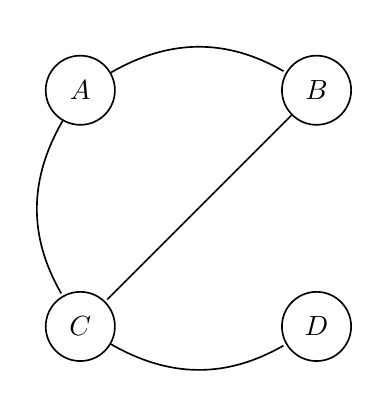
\begin{tikzpicture}[>=stealth',shorten >=1pt,auto,node distance=3cm,semithick]
  \tikzstyle{every state}=[draw=black,text=black]

  \node[state]         (A)                    {$A$};
  \node[state]         (B) [right of=A]       {$B$};
  \node[state]         (C) [below of=A]       {$C$};
  \node[state]         (D) [right of=C]       {$D$};
  
  \path (A) edge  [bend left]   node {}  (B)
            edge  [bend right]  node {}  (C)
        (B) edge                node {}  (C)
        (C) edge  [bend right]  node {}  (D);
\end{tikzpicture}}

\newcommand{\ejemplografocompleto}{
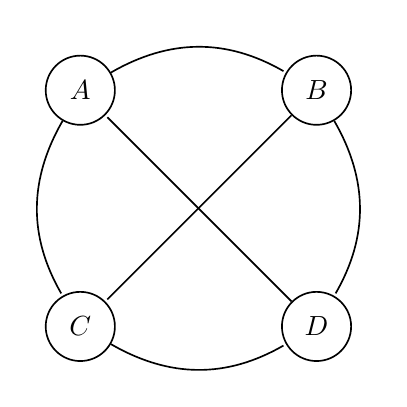
\begin{tikzpicture}[>=stealth',shorten >=1pt,auto,node distance=3cm,semithick]
  \tikzstyle{every state}=[draw=black,text=black]

  \node[state]         (A)                    {$A$};
  \node[state]         (B) [right of=A]       {$B$};
  \node[state]         (C) [below of=A]       {$C$};
  \node[state]         (D) [right of=C]       {$D$};
  
  \path (A) edge  [bend left]   node {}  (B)
            edge  [bend right]  node {}  (C)
		(B) edge  [bend left]   node {}  (D)
        (B) edge                node {}  (C)
        (D) edge                node {}  (A)
        (C) edge  [bend right]  node {}  (D);
\end{tikzpicture}}

\newcommand{\ejemplografodirigido}{
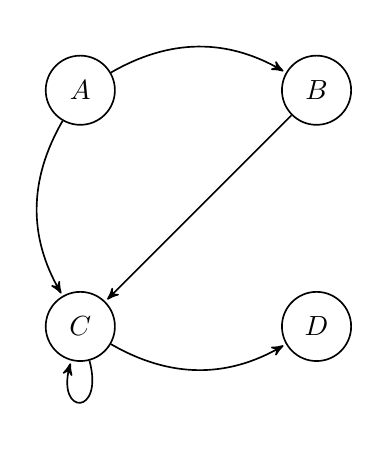
\begin{tikzpicture}[->,>=stealth',shorten >=1pt,auto,node distance=3cm,semithick]
  \tikzstyle{every state}=[draw=black,text=black]

  \node[state]         (A)                    {$A$};
  \node[state]         (B) [right of=A]       {$B$};
  \node[state]         (C) [below of=A]       {$C$};
  \node[state]         (D) [right of=C]       {$D$};
  
  \path (A) edge  [bend left]   node {}  (B)
            edge  [bend right]  node {}  (C)
        (B) edge                node {}  (C)
        (C) edge  [bend right]  node  {}  (D)
        (C) edge  [loop below]  node  {}  (C);
\end{tikzpicture}}

\newcommand{\ejemplosubgrafo}{
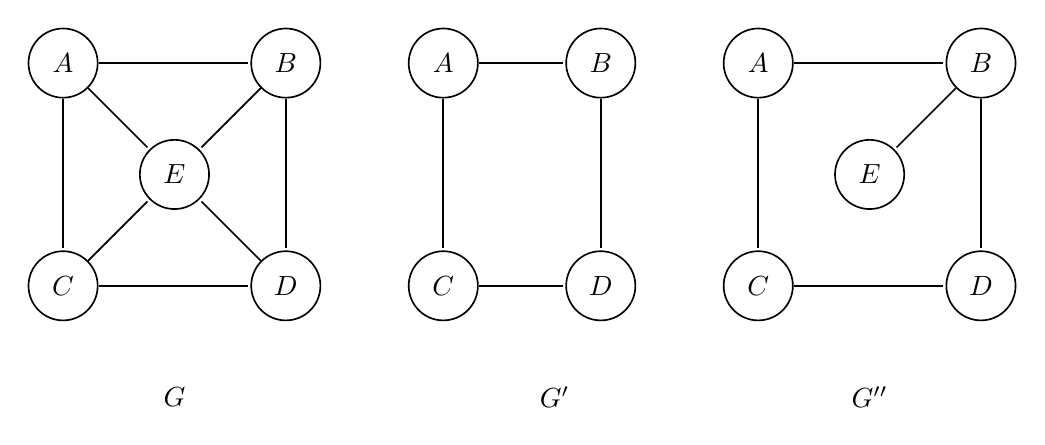
\begin{tikzpicture}[>=stealth',shorten >=1pt,auto,node distance=2cm,semithick]
  \tikzstyle{every state}=[draw=black,text=black]

% Grafo G
  \node[state]         (E)                          {$E$};
  \node[state]         (B) [above right of=E]       {$B$};
  \node[state]         (A) [above left of= E]       {$A$};
  \node[state]         (C) [below left of= E]       {$C$};
  \node[state]         (D) [below right of=E]       {$D$};

  \path (A) edge                node {}  (B)
        (A) edge                node {}  (E)
        (A) edge                node {}  (C)
        (B) edge                node {}  (D)
        (B) edge                node {}  (E)        
        (C) edge                node {}  (E)
        (C) edge                node {}  (D)
        (D) edge                node {}  (E);
        
        
% Subgrafo G'
  \node[state]         (F) [right of= B]       {$A$};
  \node[state]         (G) [right of= F]       {$B$};
  \node[state]         (H) [right of= D]       {$C$};
  \node[state]         (I) [right of= H]       {$D$};
  
  \path (F) edge                node {}  (G)
        (F) edge                node {}  (H)
        (G) edge                node {}  (I)
        (H) edge                node {}  (I);
        
% Subgrafo G'

  \node[state]         (J) [right of= G]             {$A$};
  \node[state]         (K) [right of= I]             {$C$};
  \node[state]         (N) [above right of= K]       {$E$};
  \node[state]         (M) [below right of= N]       {$D$};
  \node[state]         (L) [above right of= N]       {$B$};
  
  \path (J) edge                node {}  (K)
        (J) edge                node {}  (L)
        (L) edge                node {}  (N)
        (L) edge                node {}  (M)
        (K) edge                node {}  (M);
        
% Etiquetas con el nombre de los grafos
  \node[align=center, below right of=C] {$G$};
  \node[align=center, below right of=H] {$G'$};
  \node[align=center, below right of=K] {$G''$};
\end{tikzpicture}}

\newcommand{\ejemplounionintersecciongrafo}{
\begin{tikzpicture}[>=stealth',shorten >=1pt,auto,node distance=2cm,semithick]
  \tikzstyle{every state}=[draw=black,text=black]

% Grafo G
  \node[state]         (A)                          {$A$};
  \node[state]         (B) [below right of=A]       {$B$};
  \node[state]         (C) [below      of= B]       {$C$};
  \node[state]         (D) [right of=B]             {$D$};
  \node[state]         (E) [right of=C]             {$E$};

  \path (A) edge                node {}  (B)
        (B) edge                node {}  (C)
        (B) edge                node {}  (D)      
        (C) edge                node {}  (E)
        (D) edge                node {}  (E);
        
% Grafo G'
  \node[state]         (H) [right of= E]       {$C$};
  \node[state]         (I) [right of= D]       {$D$};
  \node[state]         (G) [right of= H]       {$E$};
  \node[state]         (F) [above right of= G] {$F$};
  
  \path (H) edge                node {}  (I)
        (I) edge                node {}  (F)
        (G) edge                node {}  (F)
        (H) edge                node {}  (G);
        
% Etiquetas con el nombre de los grafos
  \node[align=center, below right of=C] (Z) {$G$};
  \node[align=center, below right of=H] (Y) {$G'$};

% Grafo G \cup G'
  \node[state]         (J) [below left of=Z]        {$A$};
  \node[state]         (K) [below right of=J]       {$B$};
  \node[state]         (L) [below of= K]            {$C$};
  \node[state]         (M) [right of=K]             {$D$};
  \node[state]         (N) [right of=L]             {$E$};
  \node[state]         (R) [above right of=N]       {$F$};

  \path (J) edge                node {}  (K)
        (K) edge                node {}  (L)
        (K) edge                node {}  (M)      
        (L) edge                node {}  (N)
        (L) edge                node {}  (M)
        (N) edge                node {}  (R)
        (R) edge                node {}  (M)
        (M) edge                node {}  (N);
        
  \node[align=center, below right of=L] {$G \cup G'$};
  
% Grafo G \cup G'
  \node[state]         (O) [right of=R]        {$C$};
  \node[state]         (P) [right of=O]              {$E$};


  \path (O) edge                node {}  (P);
        
        
  \node[align=center, below right of=O] {$G \cap G'$};

\end{tikzpicture}}


\newcommand{\ejemplomarkov}{
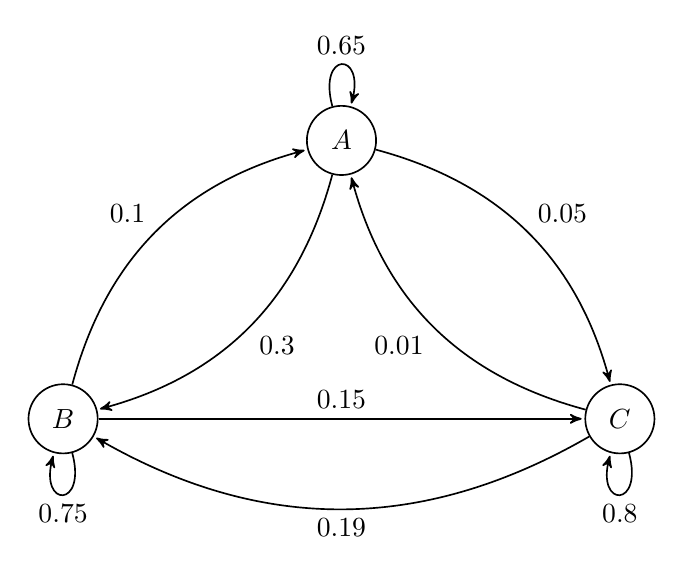
\begin{tikzpicture}[->,>=stealth',shorten >=1pt,auto,node distance=5cm,semithick]
  \tikzstyle{every state}=[draw=black,text=black]

  \node[state]         (A)                    {$A$};
  \node[state]         (B) [below left of=A]  {$B$};
  \node[state]         (C) [below right of=A] {$C$};
  
  \path (A) edge  [loop above] node {$0.65$} (A)
            edge  [bend left]  node {$0.3$}  (B)
            edge  [bend left]  node {$0.05$} (C)
        (B) edge  [loop below] node {$0.75$} (B)
            edge  [bend left]  node {$0.1$}  (A)
            edge               node {$0.15$} (C)
        (C) edge  [loop below] node {$0.8$}  (C)
            edge  [bend left]  node {$0.01$} (A)
            edge  [bend left]  node {$0.19$} (B);
\end{tikzpicture}}

\newcommand{\ejemplomarkovcompleto}{
\begin{tikzpicture}[->,>=stealth',shorten >=1pt,auto,node distance=5cm,semithick]
  \tikzstyle{every state}=[draw=black,text=black]

  \node[state]         (S)                    {$S$};
  \node[state]         (H)      [right of=A]  {$H$};
  
  \path (S) edge  [loop above] node {$0.5$}  (S)
            edge  [bend left]  node {$0.5$}  (H)
        (H) edge  [loop below] node {$0.75$} (H)
            edge  [bend left]  node {$0.25$} (S);

\end{tikzpicture}}

